\subsection{Sketch}
From a macroscopic view, the sketch is organized as a distributed prefix tree. All descendant nodes -- \emph{sketchlets} -- are responsible for a particular geospatial scope and share a common prefix with their parent. One of our primary goals behind \textsc{Synopsis} is to ensure the sketch is performant, flexible, and amenable to scaling. The sketch initiates scale-out operations to relieve memory pressure and preserve performance, while scale-in operations conserve memory. Further, any sketchlet may serve as the \emph{conduit} for queries or analytic operations.

The geohash algorithm plays a central role in the organization of the distributed sketch. Since locations are represented by bounding boxes, the algorithm facilitates collocation of observations from particular geographical scopes. This allows the conduit to redirect queries effectively and ensure data locality. Increases in the length of the geohash string correspond to geographically smaller (and more precise) bounding boxes. This is well-aligned with dynamic scaling performed by the sketch to manage memory requirements. Scaling operations within the sketch are targeted; scaling out targets geospatial locations with increased density of observations to relieve memory pressure and alleviate performance bottlenecks, while scaling in targets geolocations where there is a sparsity in available data to conserve memory.


Each sketchlet is responsible for real-time organization, summarization, and compaction of observational data from the geographical scope represented by its geohash. The sketchlet performs two operations: first, it extracts metadata from incoming observations, including geolocations, chronological information, and features encapsulated within the observation. Second, the sketchlet is responsible for summarization and compaction of the extracted features.

The sketchlet organizes its summarization in a data structure called SIFT (Summarization Involving a Forest of Trees). The edges and vertices within each SIFT tree maintain inter-feature relationships, while leaves contain online, in-memory summary statistics and correlation information to support statistical queries and generation of synthetic datasets.  The number of edges at each level within the subtrees corresponds to density-based dynamic binning of a particular feature to reduce error. The underlying principle within this data structure is \textbf{grouping} to exploit similarities in values reported within observations; grouping allows us to preserve fidelity of the observational space while conserving memory.

A simplified version of the distributed sketch for geospatial region \emph{D} is depicted in Figure~\ref{fig:dist-sketch}. Each tree within the SIFT is rooted at a higher precision geohash than that associated with the sketchlet. For example, at a sketchlet with a geohash prefix, \emph{DJ}, the trees within the SIFT at that sketchlet are rooted at higher precision geohashes such as \emph{DJB}, \emph{DJC}, \emph{DJF}, etc. An advantage of this approach is that the sketchlet partitions data from the overall geospatial scope into smaller regions, further improving the grouping of observations.

\begin{figure}
    \centerline{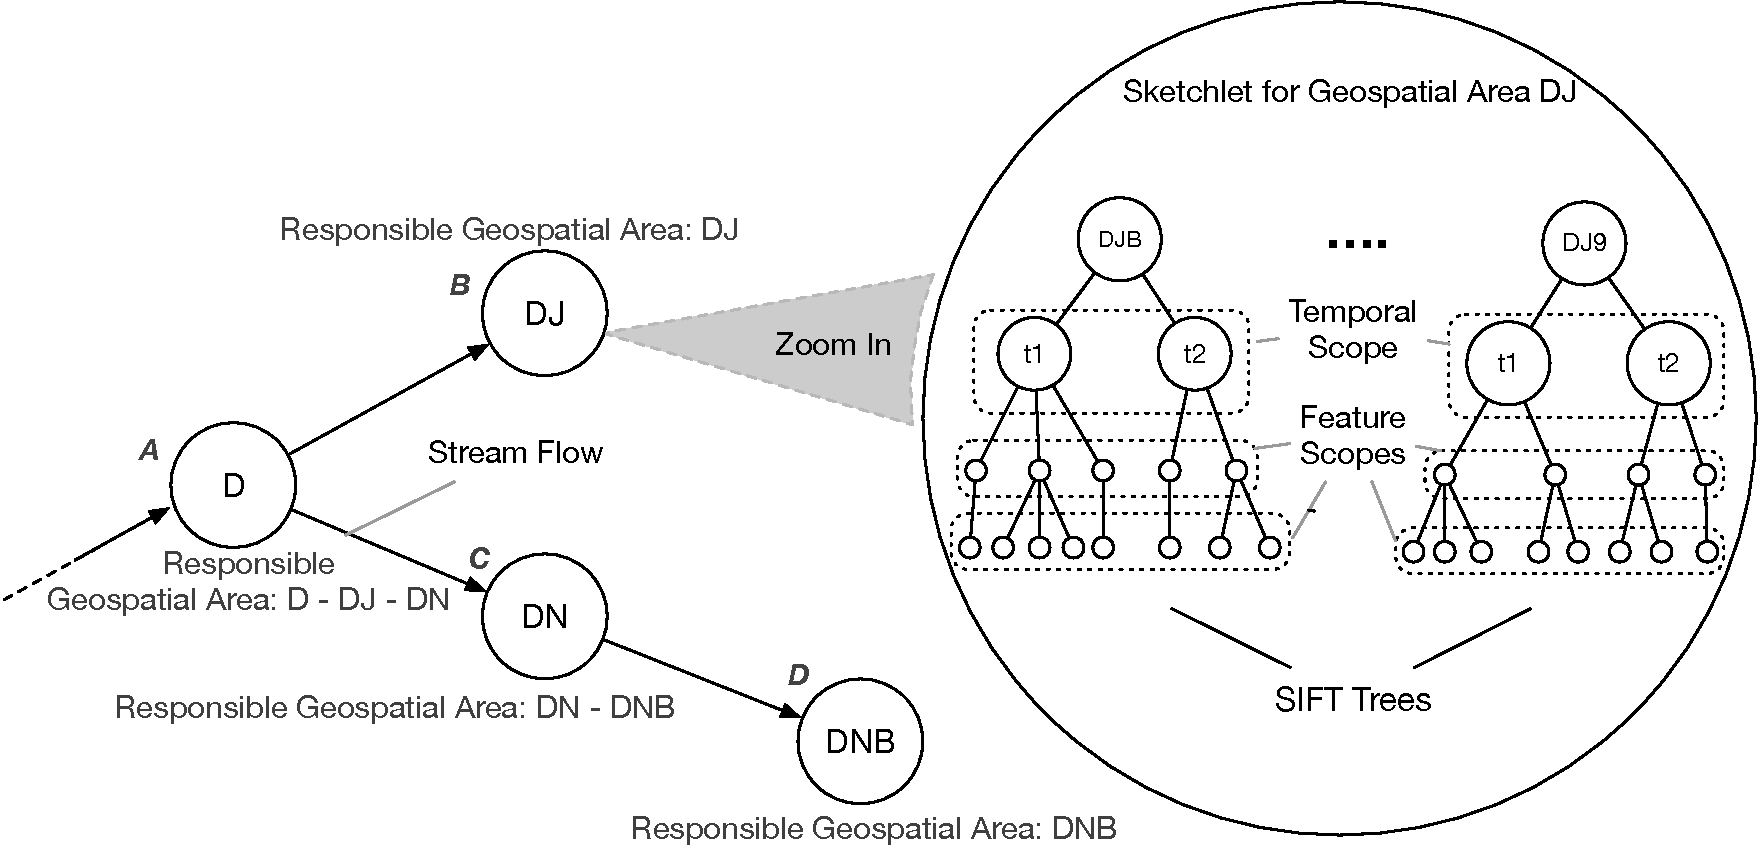
\includegraphics[width=0.5\textwidth]{figures/dist-sketch.pdf}}
    \caption{A demonstration of the distributed sketch for geohash prefix D. The sketchlets for prefixes DJ and DN have scaled out due to high volume of observations. Each sketchlet maintains a SIFT, with each tree responsible for a geospatial subregion. \vspace{-1em}}
    \label{fig:dist-sketch}
\end{figure}

The second level of the SIFT is used to group observations based on their temporal properties. This approach allows us to exploit similarity in readings reported for a particular time range. Note that as the trees are traversed, this organization strategy means that all descendants of a temporal node correspond to measurements reported for a particular region and for a particular temporal scope. The SIFT data structure also supports finer-grained temporal resolutions for the recent past -- e.g., minutes, hours, day, weeks, etc. -- along with targeted compaction operations that fold finer-grained temporal scopes into a coarser grained scopes as time advances. Specifically, our organizational structure allows us to support varying levels of expressiveness for different temporal scopes, with recent observations being represented more expressively.% For example, on 3/2/2017 we may maintain subtrees at the minute level for 3:01 pm, 3:02 pm, etc., at 3/2/2017 @ 5:00 pm these subtrees will be folded into observations for the hourly temporal scope for 3:00-4:00 pm, and at 4:00 pm the next day (3/3/2017) these would then be folded into the coarser gained temporal bin for the previous day. 

The grouping concept also extends to individual features. Each feature occupies a level within an individual tree in SIFT. At each level, the range of values that a feature can take is broken up into a set of bins (corresponding to the range of values) that they take. These ranges are determined using kernel density estimation (KDE) to ensure that the binning of features is representative of the observed density in the distribution of values for that feature at the particular spatiotemporal scope. Each node (or bin) maintains the min, max, standard deviation, mean, and the total number of observations it is responsible for.  This is useful during the creation of synthetic datasets that are representative of the observational space for a particular spatiotemporal scope.

The methodology behind SIFT accomplishes two key objectives: first, it captures the distribution of feature values across a spatiotemporal scope. Second, it supports targeted reductions in the observational data volumes while being representative of the observed feature values. This is in contrast to a random sampling scheme, which may be unable to recreate distributions with high fidelity for arbitrary spatiotemporal scopes.

The organization of the sketchlet is such that it is amenable to scale-out and scale-in operations of the distributed sketch. A key feature provided by the SIFT data structure is support for scaling operations. For example, if a subregion represented by a tree within the forest maintained at each sketchlet has a higher density (and variability) of the reported observational values, that tree would have a correspondingly higher memory footprint within the data structure. This allows us to target scaling maneuvers to particular subregions managed at a sketchlet to alleviate memory pressure.  During scale-in operations, descendants can be folded into the parent; the descendant's SIFT is simply added as a tree to the SIFT maintained at the parent.
%
\vspace{0.7em}\\
%
\textbf{Systems View of the Sketch:} The \textsc{Synopsis} sketch, comprising sketchlets dispersed over multiple machines, is a compact and memory-resident surrogate for the entire observational space. The sketch may be used for any purpose that regular, on-disk data is used for including but not limited to query evaluations, assessing statistical properties of the data, and launching computations using well-known analytical engines. The sketch is adaptive and evolves over time, with the number of sketchlets varying as scaling maneuvers occur to cope with data volumes and memory management. The structure of the SIFT also varies over time as temporal scopes are aggregated, features binned, and scaling occurs.
